\chapter{The Problem}\label{ch:problem}

\section{From Weyl to Yang and Mills}

The idea that a physical law should be unchanged when a phase is altered independently at every point of spacetime goes back to Hermann Weyl~\cite{We29}. His 1918 attempt to unify gravitation and electromagnetism through a local change of scale failed, but in 1929 he recast it as a local change of phase. The wave function $\psi(x)$ of a charged particle may be replaced by $e^{i\alpha(x)}\psi(x)$ provided the electromagnetic potential $A_\mu$ shifts by $\partial_\mu\alpha$. Invariance under this local symmetry forces the existence of the photon, and Maxwell's equations follow.

In 1954 Yang and Mills~\cite{YM54} asked what happens when the phase $e^{i\alpha(x)}$ is replaced by a matrix in a nonabelian group such as SU(2), the group that rotates the proton into the neutron. The potential becomes a matrix valued one form $A=A_\mu\,\mathrm dx^\mu$ taking values in the Lie algebra $\mathfrak g$, and the field strength becomes
\[
F_{\mu\nu}=\partial_\mu A_\nu-\partial_\nu A_\mu+[A_\mu,A_\nu].
\]
The commutator is the new ingredient: it makes the field carry the very charge it couples to, so that the equations of motion are nonlinear even without matter. The Euclidean action is
\[
S(A)=-\frac{1}{2g^2}\int_{\R^4}\operatorname{tr}\big(F_{\mu\nu}F_{\mu\nu}\big)\,\mathrm d^4x ,
\]
and it is invariant under gauge transformations $A\mapsto UAU^{-1}+U\,\mathrm dU^{-1}$ with $U(x)\in G$.

Pauli raised the obvious objection at once. Classically the theory has massless waves, so its force should have infinite range, like electromagnetism. The strong force has a range of about $10^{-15}$ metres. For a decade the equations looked beautiful and useless.

\section{Asymptotic freedom and confinement}

Three developments rescued the theory. In 1971 't Hooft~\cite{tH71a,tH71} proved that Yang Mills theories are renormalizable. In 1973 Gross and Wilczek~\cite{GW73}, and independently Politzer~\cite{Po73}, computed how the coupling depends on the momentum scale $k$ and found that it decreases at short distances. For SU(N) without matter the one loop running is
\[
k\frac{\mathrm dg}{\mathrm dk}=-b_0g^3+O(g^5),\qquad b_0=\frac{11N}{48\pi^2},
\]
so that the coupling vanishes logarithmically as the distance scale shrinks. This is asymptotic freedom\index{asymptotic freedom}. Its consequence at long distances is equally important: the coupling grows, and perturbation theory loses control at the scale
\[
\Lambda=k\exp\Big(-\frac{1}{2b_0g(k)^2}\Big)\big(1+\dots\big),
\]
which is the only scale in pure Yang Mills theory. Every mass in the theory, if there is one, must be a pure number times $\Lambda$.

In 1974 Wilson~\cite{Wi74} put the theory on a lattice. Gauge fields become group elements $U_\ell\in G$ on the links of $\Z^4$, and the action becomes a sum over plaquettes,
\[
S_W(U)=\frac{\beta}{N}\sum_p\Big(N-\operatorname{Re}\operatorname{tr}U_p\Big),\qquad \beta=\frac{2N}{g^2},
\]
where $U_p$ is the ordered product of the four link variables around the plaquette $p$. Wilson showed that at strong coupling, where $\beta$ is small, the expectation of a large rectangular loop decays like the exponential of its area. That area law means a linearly rising potential between static charges, which is confinement\index{confinement}. In 1980 Creutz~\cite{Cr80} began the numerical study of the lattice theory by Monte Carlo and found that the strong coupling behaviour passes smoothly into the weak coupling regime governed by asymptotic freedom, with no phase transition in between for SU(2). The modern lattice glueball\index{glueball} spectrum, computed by Morningstar and Peardon~\cite{MP} among others, has a lightest scalar state of mass about $1.7$ GeV in SU(3), several further stable states below the two glueball threshold, and a rich tower above it.

None of this is a proof. Lattice Monte Carlo is numerical evidence on finite lattices at finite spacing, and the strong coupling expansion converges only for small $\beta$, far from the continuum limit $\beta\to\infty$.

\section{The Millennium Prize Problem}

In 2000 the Clay Mathematics Institute listed the following problem, in the formulation of Jaffe and Witten~\cite{JW}.

\begin{quote}
Prove that for any compact simple gauge group $G$, a nontrivial quantum Yang Mills theory exists on $\R^4$ and has a mass gap\index{mass gap} $\Delta>0$.
\end{quote}

Existence means the construction of a quantum field theory satisfying axioms at least as strong as those of Wightman, or equivalently of Osterwalder and Schrader\index{Osterwalder, K.!and Schrader, R.}~\cite{OS} in Euclidean form, whose short distance behaviour is that of asymptotically free perturbation theory. The mass gap means that the Hamiltonian $H$ of the theory has spectrum
\[
\operatorname{spec}H\subset\{0\}\cup[\Delta,\infty),
\]
with a unique vacuum $\Omega$ at $0$. Equivalently, for every gauge invariant local observable $O$ with $\langle O\rangle=0$, the connected Euclidean correlation decays exponentially:
\[
\big|\langle O(\tau)O(0)\rangle\big|\le K_O\,e^{-\Delta\tau}.
\]
The correlation length is $1/\Delta$.

\section{The status in 2026}

Constructive quantum field theory built interacting theories in two and three dimensions in the 1970s; Glimm and Jaffe's construction of $\phi^4_3$~\cite{GJ} is the landmark. In four dimensions the most complete rigorous work on gauge theories before 2026 was Ba\l aban\index{Balaban, T.@Ba\l aban, T.}'s renormalization group analysis of lattice gauge theory~\cite{Ba87}, which established ultraviolet stability, and the construction of SU(2) Yang Mills in finite volume with an infrared cutoff by Magnen, Rivasseau and S\'eneor~\cite{MRS}.

On 26 October 2026 OpenAI announced~\cite{OAI} that its models had produced a proof of the existence half of the problem, with a natural language proof dated 9 September and a Lean formalisation completed on 16 October. A review group led by David Gross endorsed the existence part, and on 10 November 2026 released the Lean code together with a validation assessment, describing the result as the existence of pure Yang Mills theory according to established definitions and stating that confinement and the mass gap remain open.

Section~\ref{sec:existence2026} records what was announced and what was not. We do not use the details of that construction in this book. What matters for us is the logical situation it leaves behind. The existence of a theory satisfying the Osterwalder Schrader axioms is now claimed, though not yet independently checked, and with it the reconstruction of a Hilbert space, a vacuum and a positive Hamiltonian. If the claim stands, the remaining question is purely spectral: is $0$ an isolated point of the spectrum of $H$?

\section{What a gap is, in the language of measures}

For any gauge invariant observable $O$ at zero spatial momentum, the spectral theorem writes the Euclidean correlation as
\[
C_O(\tau)=\langle O,e^{-\tau H}O\rangle-|\langle\Omega,O\rangle|^2=\int_{(0,\infty)}e^{-\tau E}\,\mu_O(\mathrm dE),
\]
where $\mu_O$ is a nonnegative measure, the spectral measure\index{spectral measure} of $O$. The gap for $O$ is the left edge of its support, and the gap of the theory is the infimum over observables:
\[
\Delta_O=\inf\operatorname{supp}\mu_O,\qquad \Delta=\inf_O\Delta_O .
\]
The whole problem is therefore a question about the supports of a family of positive measures, constructed as limits of lattice measures. This is the form in which a probabilist can engage with it, and it is the form we use throughout.

The measures have structure. Each $C_O$ is completely monotone in $\tau$, the measures depend on the lattice spacing $a$ and the coupling $\beta$ through a renormalization group, and asymptotic freedom fixes how $a$ must depend on $\beta$:
\[
a(\beta)\,\Lambda\propto\exp\Big(-\frac{12\pi^2}{11N^2}\,\beta\Big)\big(1+o(1)\big)
\]
at one loop, with $\beta=2N/g^2$. For SU(2) the exponent is $3\pi^2\beta/11$. A lattice gap $m(\beta)$, measured in units of the lattice spacing, gives a physical gap $\Delta=m(\beta)/a(\beta)$. Heuristically, the continuum limit has a gap exactly when $m(\beta)$ shrinks no faster than $a(\beta)$ as $\beta\to\infty$.

Figure~\ref{fig:specgap} shows the picture behind the whole book: a spectral measure with an empty interval above zero, and the exponential decay in Euclidean time that the empty interval forces.

\begin{figure}[t]
\centering
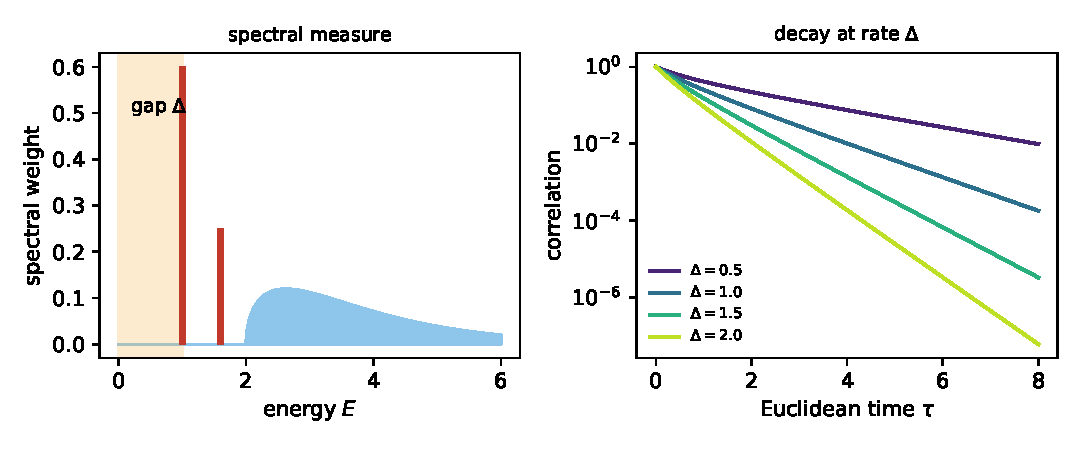
\includegraphics[width=0.95\textwidth]{figures/spectrum_gap.pdf}
\caption[A spectral measure with a gap]{Left: a spectral measure with two stable states and a continuum, and an empty interval of width $\Delta$ above the vacuum. Right: the Euclidean correlation produced by the same shape of measure shifted to four different gaps; the slope at large time is $-\Delta$.}
\label{fig:specgap}
\end{figure}

\section{The plan of the book}

The book has six parts and a closing chapter.

Chapters~\ref{ch:problem} and~\ref{ch:positivity} (Part I) set up lattice gauge theory as a probability model, explain where positivity comes from, and collect the Thorin toolkit. Chapters~\ref{ch:routeA} to~\ref{ch:hitting} (Part II) translate the gap into statements about generalized gamma convolutions along two routes, treat the gap as a parameter to estimate, and are about computation and the people whose ideas it rests on: latent variables and nested sampling, the vertical likelihood family and split sampling, Yakowitz's weighted Monte Carlo, Kac and P\'olya on models, Jerrum and Sinclair on randomised approximation, Sokal on autocorrelation, clusters and zeros, slice variables, log concavity and Besag's Markov random fields, and hitting times as a way to learn the gap. Section~\ref{ch:plgbc} applies sufficient statistics, particle learning and generative Bayesian computation to the ladder.

Chapter~\ref{ch:twod} (Part III) holds the solvable worlds: two dimensions, with a guided tour, the Riemann kernel on the three sphere, dynamic and static gaps, the renormalization group for statisticians, free fields, and large $N$.

Chapters~\ref{ch:strong} to~\ref{ch:theta} (Part IV) go to four dimensions, through strong coupling, lattice Monte Carlo for glueballs, the Migdal Kadanoff ladder and its verification, the ladder on counts and Kingman's coalescent, real zeros, and theta kernels, fermion determinants and Howe duality.

Chapters~\ref{ch:path} to~\ref{ch:sandwich} (Part V) are the path that remains and new work on the open problems: Sections~\ref{ch:isthere} and~\ref{ch:missing} assess the path and what it leaves out, and the chapters give a product formula for the SU(2) heat kernel that closes, for SU(2), the likelihood ratio problem, tests of the ladder against lattice data, an empirical sandwich between two caricatures in three and four dimensions, correlation inequalities, and the case for three dimensions first. Chapter~\ref{ch:kacyang} (Part VI), Neighbouring Problems, takes up Kac and Yang's discrete system, stochastic quantisation and filtering, Hilbert's sixth problem, and what this book owes to our Riemann and Langlands volumes. Chapter~\ref{ch:programme} lists twelve problems in order of difficulty, Section~\ref{ch:history} gives the history, and Section~\ref{ch:results} summarises what is new. The appendices contain the code, auxiliary proofs, notation, a dictionary between the languages of physics and statistics, solutions, a computational notebook and a glossary.

\section{Results at a glance}

\begin{center}
\scriptsize
\begin{tabular}{p{2.55in}p{0.85in}p{0.6in}}
\toprule
result & status & where \\ \midrule
spectral measure is a Thorin measure\index{Thorin measure}; gap is the tail index of a GGC~\cite{Th77} & theorem & Ch.~\ref{ch:routeA} \\
$2\sin^2$ transport is unconditional; Thorin density\index{Thorin density} is a L\'evy exponent\index{Levy exponent@L\'evy exponent} & theorem & Sec.~\ref{ch:routeB} \\
gap is the decay rate of the Thorin densities; constant in the uniform inequality is free & theorem & Sec.~\ref{ch:routeB} \\
correlators with two isolated levels are not GGC & theorem & Sec.~\ref{ch:routeB} \\
gap estimated as a support constraint in positive deconvolution\index{positive deconvolution} & numerical & Ch.~\ref{ch:estimation} \\
2D SU(2): $\Delta(a)\ge\Delta_{\mathrm{cont}}\operatorname{arcsinh}(x)/x$ at every spacing & theorem & Ch.~\ref{ch:twod} \\
Riemann's $\Phi$ from the return density of Brownian motion\index{Brownian motion on SU(2)} on $S^3$ & theorem & Sec.~\ref{ch:riemann} \\
Migdal Kadanoff preserves positive definiteness & theorem & Sec.~\ref{ch:mk} \\
MK decrement $(1-b^{-2})N^2\E S_{\mathrm{BPY}}/4$, within $3\%$ of one loop at $b=2$ & leading order & Sec.~\ref{ch:mk} \\
SU(3) decrement approaches $9/16$ & numerical & Sec.~\ref{ch:mk} \\
MK map monotone from a likelihood ratio\index{likelihood ratio order} property & theorem & Sec.~\ref{ch:verification} \\
decrement of the SU(2) heat kernel projected ladder positive at every coupling & theorem & Ch.~\ref{ch:progress} \\
correlation length as a first passage time\index{first passage time} & derivation & Sec.~\ref{ch:verification} \\
product formula for the SU(2) heat kernel; likelihood ratio property at every time & theorem & Ch.~\ref{ch:progress} \\
weak coupling expansion of the ladder to three orders; two loop ratio $1/(6b^2)$ & theorem & Ch.~\ref{ch:progress} \\
convolution is totally positive when $\Delta f/f$ is monotone & theorem & Ch.~\ref{ch:progress} \\
gap as Poincar\'e constant of the ground state measure & proposition & Sec.~\ref{ch:h6ym} \\
ladder against lattice data: rate within $15\%$, crossover misplaced & numerical & Ch.~\ref{ch:progress} \\
vertical likelihood, split sampling, nested sampling on exact 2D torus & numerical & Sec.~\ref{ch:vertical} \\
Yakowitz rate $n^{-2}$ in thermodynamic integration & numerical & Sec.~\ref{ch:yakowitz} \\
dynamic gap equals static gap; log Sobolev route & survey & Sec.~\ref{ch:dynamic} \\
empirical sandwich: loop laws between independent and MK caricatures & numerical & Ch.~\ref{ch:sandwich} \\
upper half of the sandwich for expectations, $W_{22}\ge W_{11}^4$, any compact group & theorem & Sec.~\ref{ch:griffiths} \\
particle learning of the decrement; GBC matching of blocked ensembles & numerical & Sec.~\ref{ch:plgbc} \\
\bottomrule
\end{tabular}
\end{center}

\begin{center}
\scriptsize
\begin{tabular}{p{2.55in}p{0.85in}p{0.6in}}
\toprule
result & status & where \\ \midrule
coalescence of the latent count is hypergeometric; Kingman duality & theorem & Ch.~\ref{ch:counts}, Sec.~\ref{ch:kingman} \\
the count is $E[1/(1-\cos\theta)]-2$; first rung drift tending to $-\frac{13}{16}$ from point masses and to $+\frac18$ from Wilson laws; the heat kernel value $-\frac12$ is numerical & theorem, numerical & Ch.~\ref{ch:counts} \\
real zeros under heat flow; smoothed criterion for convolutions & theorem & Ch.~\ref{ch:zeros} \\
closure of the real zeros class under convolution & conjecture & Ch.~\ref{ch:zeros} \\
Hartman Watson law is a generalized gamma convolution & theorem & Ch.~\ref{ch:zeros} \\
vacuum of one plaquette has real zeros; rule for registers & theorem, numerical & Sec.~\ref{ch:quantum} \\
fermion determinants, matching expansion of decimation & theorem & Ch.~\ref{ch:theta} \\
comparison of MK with $\Z^4$ at the level of spectral measures & open & Sec.~\ref{ch:isthere} \\
\bottomrule
\end{tabular}
\end{center}

Two warnings. No chapter proves the mass gap. And the Migdal Kadanoff recursion, which carries the four dimensional analysis, is exact only on hierarchical lattices; its relation to the true theory on $\Z^4$ is the central open problem of Chapter~\ref{ch:path}.

\section{Gauge theory for probabilists}\label{ch:gauge}

Lattice gauge theory is a probability model: a random field of group elements on the edges of a graph, with a Gibbs density invariant under a large symmetry group. Nothing here is new, but the probabilistic vocabulary is the one we use throughout.

\subsection{Random group elements on edges}

Let $G$ be a compact Lie group, for us SU(2) or SU(3), with normalised Haar measure\index{Haar measure} $\mathrm dU$. Let $B$ be a finite box in $\Z^d$ with periodic boundary conditions, and let $\mathcal E(B)$ be a set of links containing one orientation of each edge. A gauge field configuration assigns a group element $U_\ell\in G$ to every link $\ell$, with the convention $U_{\ell^{-1}}=U_\ell^{-1}$ for the reversed link. The configuration space is the product $G^{\mathcal E(B)}$, a compact manifold of dimension $\dim G\cdot|\mathcal E(B)|$, and the reference measure is the product Haar measure.

A plaquette $p$ is an elementary square of the lattice, with boundary links $\ell_1,\ell_2,\ell_3,\ell_4$ traversed in order. Its holonomy is the ordered product
\[
U_p=U_{\ell_1}U_{\ell_2}U_{\ell_3}U_{\ell_4}.
\]
Changing the starting corner conjugates $U_p$, and reversing the orientation inverts it. A class function of $U_p$, that is a function invariant under conjugation, is therefore well defined on unoriented plaquettes if it is also invariant under inversion.

\begin{definition}
A lattice gauge theory with plaquette weight $f$, a positive class function on $G$ with $f(U^{-1})=f(U)$, is the probability measure
\[
\mathbb P_B(\mathrm dU)=\frac{1}{Z_B}\prod_pf(U_p)\prod_\ell\mathrm dU_\ell
\]
on $G^{\mathcal E(B)}$.
\end{definition}

The Wilson weight is $f(U)=\exp(\frac\beta N\operatorname{Re}\operatorname{tr}U)$ for SU(N). The heat kernel\index{heat kernel} weight is the density of Brownian motion\index{Brownian motion on SU(2)} on $G$ at time $t$, evaluated at $U$.

Figure~\ref{fig:wilsonlaws} shows the law of the rotation angle of a single plaquette under the Wilson weight. At small $\beta$ it is close to Haar measure; as $\beta$ grows it concentrates at the identity, which is weak coupling.

\begin{figure}[t]
\centering
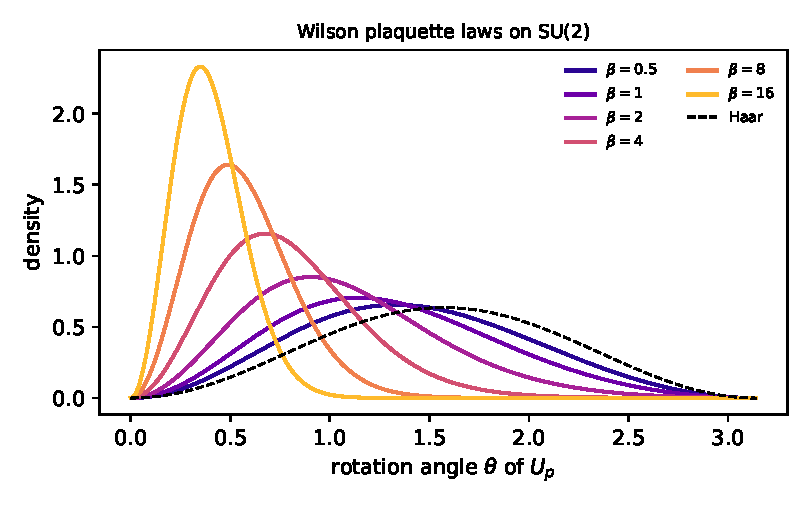
\includegraphics[width=0.85\textwidth]{figures/wilson_laws.pdf}
\caption[Wilson plaquette laws on SU(2)]{Density of the rotation angle $\theta$ of a plaquette variable under the single plaquette Wilson weight $e^{\beta\cos\theta}$ times Haar measure on SU(2), for six couplings, with the Haar density dashed.}
\label{fig:wilsonlaws}
\end{figure}

\subsection{Gauge invariance}

A gauge transformation assigns a group element $\omega_x$ to every site $x$ and acts on links by $U_{xy}\mapsto \omega_xU_{xy}\omega_y^{-1}$. Plaquette holonomies are conjugated, so class functions of them are unchanged, and Haar measure is invariant under left and right multiplication. The measure $\mathbb P_B$ is therefore invariant under the gauge group $G^{B}$, which is enormous: its dimension is comparable to that of the configuration space.

Gauge invariance has two consequences for probabilists. First, only gauge invariant observables have meaningful expectations; the expectation of any observable that is not gauge invariant is the expectation of its gauge average. On a finite box this is just the invariance of $\mathbb P_B$; Elitzur's theorem~\cite{El75} is the infinite volume statement that gauge symmetry cannot break. Second, one may fix a gauge to reduce the number of variables. In axial gauge one sets all links in one direction to the identity along a maximal tree, and, with free boundary conditions, the plaquette variables become independent in two dimensions. This is the reason two dimensional Yang Mills is solvable.

\subsection{Observables}

The basic gauge invariant observables are traces of holonomies around closed loops.
\begin{itemize}
\item The Wilson loop $W(\mathcal C)=\operatorname{tr}\prod_{\ell\in\mathcal C}U_\ell$ for a closed lattice curve $\mathcal C$. Its expectation measures the energy of a pair of static charges: for a rectangular $R\times T$ loop, $\langle W\rangle\approx e^{-V(R)T}$ for large $T$, where $V(R)$ is the static potential.
\item The plaquette observable $\operatorname{tr}U_p$, and its spatial sums at a fixed time, which project onto zero momentum glueball states. Combinations of plaquettes with definite behaviour under the lattice rotation group select the quantum numbers $J^{PC}$.
\item The Polyakov loop, the trace of the product of links along a closed curve wrapping the periodic time direction, whose expectation measures the free energy of a single static charge and serves as an order parameter for deconfinement at finite temperature.
\end{itemize}
Confinement means an area law for large Wilson loop\index{Wilson loop}s, $\langle W(\mathcal C)\rangle\le K\,e^{-\sigma\,\mathrm{Area}(\mathcal C)}$ for a constant $K$, with string tension $\sigma>0$. The mass gap\index{mass gap} concerns the correlations of local observables such as plaquettes. The two are related but distinct: in two dimensions there is confinement\index{confinement} with a string tension but no propagating particles.

\subsection{Character expansion as a Fourier expansion}

Since $f$ is a class function, it has a Fourier expansion in characters,
\[
f(U)=\sum_\lambda d_\lambda\,c_\lambda\,\chi_\lambda(U),
\]
where $\lambda$ runs over irreducible representations, $d_\lambda$ is the dimension and $\chi_\lambda$ the character. The coefficients are $c_\lambda=d_\lambda^{-1}\int f\bar\chi_\lambda\,\mathrm dU$. Two facts make this expansion the natural coordinate system.
\begin{enumerate}
\item[(i)] Convolution diagonalises: if $f*g(U)=\int f(UV^{-1})g(V)\mathrm dV$, then $c_\lambda(f*g)=c_\lambda(f)c_\lambda(g)$. Integrating out a link shared by two plaquettes in a plane is such a convolution.
\item[(ii)] Products decompose by Clebsch Gordan: $\chi_\kappa\chi_\nu=\sum_\lambda n^\lambda_{\kappa\nu}\chi_\lambda$ with nonnegative integer multiplicities $n^\lambda_{\kappa\nu}$.
\end{enumerate}
Writing $u_\lambda=c_\lambda/c_{\mathrm{triv}}$, the normalised coefficients satisfy $|u_\lambda|\le1$, and they equal the Fourier transform $\E[\chi_\lambda(U)]/d_\lambda$ of the probability law with density $f/c_{\mathrm{triv}}$. We call them Thorin levels in this book, because in Section~\ref{ch:mk} they play the role that the levels of the Thorin ladder play in our Riemann programme.

\subsection{Transfer matrices}

Choose one lattice direction as time. Group the links into time slices: the spatial links at time $\tau$ and the temporal links from $\tau$ to $\tau+1$. In temporal gauge, the temporal links are set to the identity, and the measure becomes a Markov chain in time whose state is the configuration of spatial links at time $\tau$, subject to Gauss's law. The transition kernel is the transfer matrix\index{transfer matrix} $\mathcal T$, an integral operator on $L^2$ of the spatial configuration space restricted to gauge invariant functions. Reflection positivity~\cite{OSe,Lu77}, discussed in Chapter~\ref{ch:positivity}, makes $\mathcal T$ selfadjoint and positive. The Markov chain picture has a simple consequence: correlations of time slice observables are matrix elements of powers of $\mathcal T$,
\[
\langle O_0O_n\rangle-\langle O\rangle^2=\langle O,\mathcal T^nO\rangle_0=\int\eta^n\,\mu_O(\mathrm d\eta),
\]
where $\mu_O$ now denotes the spectral measure\index{spectral measure} in the variable $\eta=e^{-aE}$. It lives on $[0,1)$ once $\mathcal T$ is normalised to have top eigenvalue $1$ and that eigenvalue, the vacuum, is removed. This is the Laplace transform representation of Chapter~\ref{ch:positivity}. The mass gap is the spectral gap of this Markov chain, in units of the lattice spacing: the distance between the top eigenvalue and the rest of the spectrum, measured on the logarithmic scale.

This makes the mass gap a close relative of a familiar probabilistic question, the rate of convergence to equilibrium of a Markov chain. The difference is that the chain here is infinite dimensional, its state space is the configuration of a whole spatial slice, and the question is whether the rate survives an infinite sequence of rescalings.

\subsection{Scales and the continuum limit}

The lattice measure contains no length; physical units enter only by holding a physical quantity, such as the lightest glueball mass, fixed as $\beta$ varies. Asymptotic freedom forces $\beta\to\infty$ as $a\to0$, so the continuum limit is taken along a curve in the space of lattice theories, the renormalized trajectory, on which the correlation length in lattice units diverges like $1/a$. A continuum gap means it diverges no faster. The renormalization group follows this curve by replacing a theory at spacing $a$ with an effective theory at spacing $ba$; Sections~\ref{ch:mk} and~\ref{ch:verification} study an approximation to it in which both asymptotic freedom and confinement are visible.

\section{Probabilists and gauge fields}\label{ch:probabilists}

The approach of this book is probabilistic, and it joins a line of work by probabilists on gauge theories that has grown substantially since the 1990s. This section surveys that line briefly, to place our contribution and to point the reader to results that bear on the mass gap\index{mass gap}. We describe each strand at the level of its main idea and avoid claims about details we have not checked.

\subsection{Two dimensional Yang Mills measures}

In two dimensions the continuum Yang Mills measure can be constructed directly as a probability measure on connections modulo gauge, or more precisely on the holonomies of loops. Driver~\cite{Dr89} and Sengupta constructed it in the plane and on surfaces in the late 1980s and early 1990s~\cite{Se97}, using that in two dimensions the holonomies along a family of nested loops behave like Brownian motion\index{Brownian motion on SU(2)} on the group. Thierry L\'evy~\cite{Le03} developed the theory systematically: the Yang Mills measure on a compact surface as a random holonomy process, its Markov property under cutting and gluing of surfaces, and its relation to Brownian motion on the structure group. The partition functions of Chapter~\ref{ch:twod} are the total masses of these measures, and the heat kernel\index{heat kernel} of Brownian motion on the group is their basic building block. The large $N$ limit, the master field, was studied by L\'evy and by Anshelevich and Sengupta~\cite{AS12} among others, and connects to free probability.

For our purposes the lesson is that in two dimensions gauge theory is, quite literally, the theory of Brownian motion on a compact group indexed by area. Chapter~\ref{ch:twod} uses exactly this, and Section~\ref{ch:mk} tries to carry it to four dimensions through the renormalization group.

The basic process is Brownian motion on SU(2), the three sphere. Figure~\ref{fig:s3bm} shows eight paths, recorded through their angle from the identity, and the law of that angle at time six of standard Brownian motion on the unit three sphere (generator one half the Laplacian, which is time twelve in the clock of the heat kernel $K_t$ used in this book), already close to the Haar density $\frac2\pi\sin^2\theta$. The two dimensional Yang Mills measure is built from the bridges of this process.

\begin{figure}[t]
\centering
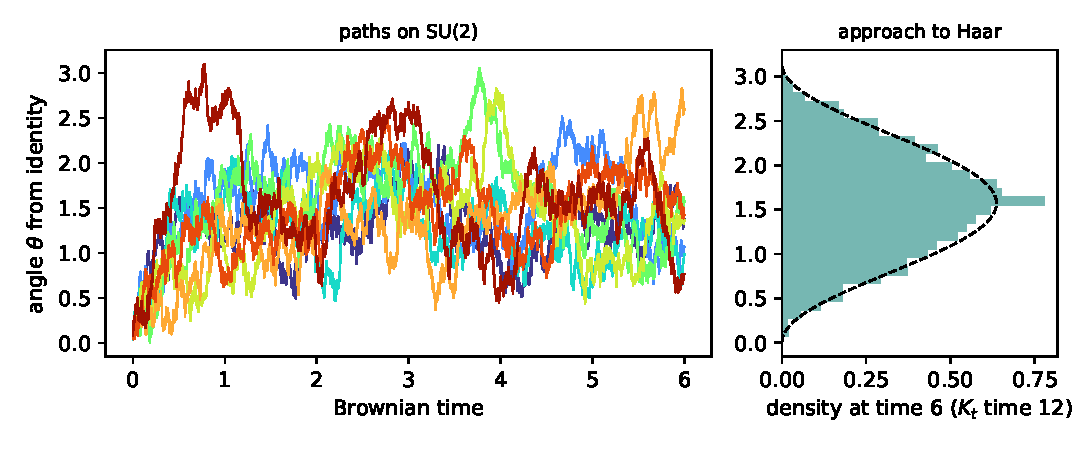
\includegraphics[width=0.95\textwidth]{figures/s3_brownian.pdf}
\caption[Brownian motion on SU(2)]{Left: eight Brownian paths on SU(2), shown through their angle from the identity. Right: the histogram of the angle at time six of standard Brownian motion (time twelve of $K_t$) from three thousand paths, against the Haar density (dashed).}
\label{fig:s3bm}
\end{figure}

\subsection{Lattice gauge theory as a probability model}

Chatterjee initiated a programme of rigorous probabilistic analysis of lattice gauge theories, with an influential survey addressed to probabilists~\cite{Ch19}. Results in this line include computations of Wilson loop\index{Wilson loop} expectations in $\Z_2$ lattice gauge theory at weak coupling, extensions by Cao~\cite{Ca20} and by Forsstr\"om, Lenells and Viklund~\cite{FLV22} to finite gauge groups, and string trajectory and surface sum representations~\cite{Ch19so,CPS25} of Wilson loop expectations at strong coupling, related to the large $N$ loop equations of Makeenko and Migdal~\cite{MM79}. Adhikari and Cao~\cite{AC} proved exponential decay of correlations, which can be read as a lattice mass gap, for lattice gauge theories with finite, possibly nonabelian, gauge groups at weak coupling.

These results are important because they treat weak coupling, the regime where the continuum limit lives, and because they are stated in probabilistic terms. The finite group case differs from the continuous group case in an essential way, however: for a finite group there is no asymptotic freedom\index{asymptotic freedom}, weak coupling is a frozen phase, and the lattice spacing does not need to shrink. The continuous group problem requires following the theory across scales, which is what the renormalization group does.

\subsection{Stochastic quantization}

A different probabilistic approach constructs the Yang Mills measure as the invariant measure of a stochastic partial differential equation, the Langevin dynamics of the Yang Mills action. Chandra, Chevyrev, Hairer and Shen constructed the Langevin dynamics for two dimensional Yang Mills, and the stochastic quantisation of three dimensional Yang Mills Higgs theory~\cite{CCHS,CCHS3}, using the theory of regularity structures~\cite{Ha14}, which handles the singular products that appear when noise is rough; Chevyrev and Shen~\cite{ChSh23} proved that the two dimensional Yang Mills measure is invariant for the renormalised dynamics. On the lattice, Shen, Zhu and Zhu~\cite{SZZ} developed a stochastic analysis approach to lattice Yang Mills at strong coupling in any dimension: Langevin dynamics, ergodicity, Poincar\'e and log Sobolev inequalities, large $N$ limits, and a mass gap for the infinite volume measure.

The stochastic quantization approach is attractive because spectral gaps of Markov dynamics are a central topic in probability, with tools such as Poincar\'e and log Sobolev inequalities and Bakry \'Emery curvature~\cite{BE}. The difficulty is that the relevant curvature is not uniformly positive in four dimensions, and controlling it is again a multiscale problem.

\subsection{Abelian theories in three dimensions}

The one complete rigorous proof of confinement\index{confinement} and a mass gap for a gauge theory at weak coupling with a nontrivial mechanism is for compact U(1) lattice gauge theory in three dimensions. Polyakov argued in 1977~\cite{Po77} that monopoles, which exist because the gauge group is compact, form a Coulomb gas whose screening gives the photon a mass and confines electric charge. G\"opfert and Mack~\cite{GM82} turned this into a theorem in 1982, proving a mass gap and an area law at all couplings. The proof is a tour de force of multiscale analysis of a Coulomb gas. It does not extend to nonabelian groups or to four dimensions, but it shows that a mass gap can be proved by following an explicit mechanism across scales.

\subsection{Hierarchical lattices}

The Migdal Kadanoff\index{Migdal Kadanoff recursion} recursion~\cite{Mi75,Ka76} used in Sections~\ref{ch:mk} and~\ref{ch:verification} is exact on hierarchical lattices, and there it has been analysed rigorously. In 1985 Ito\index{Ito, K. R.}~\cite{Ito85} proved permanent quark confinement, an area law at all couplings, for four dimensional hierarchical lattice gauge theories of Migdal Kadanoff type. Tomboulis\index{Tomboulis, E. T.}~\cite{To07} later tried to carry such bounds to $\Z^4$ by bracketing the true partition functions between Migdal Kadanoff type decimation\index{decimation}s; Ito and Seiler~\cite{IS} identified gaps in that argument in 2007 and 2008, and Tomboulis replied. Our analysis in Sections~\ref{ch:mk} and~\ref{ch:verification} works inside the same approximation and should be read against Ito's theorem: what it adds is a spectral and quantitative reading, not confinement on the hierarchical lattice itself.

\subsection{The renormalization group}

Ba\l aban\index{Balaban, T.@Ba\l aban, T.}'s series of papers in the 1980s built a rigorous renormalization group for lattice gauge theories in three and four dimensions, based on block spin transformations that average link variables over blocks and on a careful separation of small field and large field regions. It establishes ultraviolet stability: bounds on the effective actions that are uniform in the lattice spacing in the weak coupling regime. Magnen, Rivasseau and S\'eneor~\cite{MRS} constructed four dimensional SU(2) Yang Mills in a finite volume with an infrared cutoff by related methods. In both cases the analysis controls the flow from short distances down to a fixed physical scale, but not the flow into the strong coupling regime that generates the gap.

\subsection{The 2026 existence proof}

The announced 2026 existence proof is described in Section~\ref{sec:existence2026}. We treat its announced existence of a continuum theory satisfying the axioms as a working hypothesis and do not rely on the details.

\subsection{Where this book sits}

Against this background, our contribution is narrower and more specific than any of the programmes above. We do not construct measures and we do not prove a mass gap. We offer a translation of the mass gap into statements about generalized gamma convolution\index{generalized gamma convolution}s and Thorin measure\index{Thorin measure}s, built on reflection positivity\index{reflection positivity}; an exact two dimensional theorem in that language; a product formula for the SU(2) heat kernel, a coalescent description of the latent counts, and results on real zeros; a probabilistic reading of the Migdal Kadanoff renormalization group in which asymptotic freedom is the mean of a Biane Pitman Yor\index{Biane Pitman Yor variable}~\cite{BPY} variable; and a precise formulation of what would have to be compared to complete the argument. The approaches surveyed in this section are natural sources of the tools that comparison will need: L\'evy's holonomy processes for two dimensional building blocks, Ba\l aban's block spins for the true flow, and the curvature methods of stochastic quantization for the likelihood ratio\index{likelihood ratio order} comparisons of Chapter~\ref{ch:path}.
